% REMEMBER: You must not plagiarise anything in your report. Be extremely careful.
\documentclass{l4proj}
    
%==============================================================================
% Put any additional packages here
% You can add any packages you want, as long as it does not alter
% the overall format (e.g. don't change the margins or the reference style).
%
\usepackage{pdfpages} % if you want to include a PDF for an ethics checklist, for example
%
%

\begin{document}

%==============================================================================
%% METADATA
\title{Investigating students affective states in CS1 labs using affective survey software
}
\author{Evie Stokes}
\date{{\today}}

\maketitle

%==============================================================================
%% ABSTRACT
\begin{abstract}
    Every abstract follows a similar pattern. Motivate; set aims; describe work; explain results.
    \vskip 0.5em
    ``XYZ is bad. This project investigated ABC to determine if it was better. 
    ABC used XXX and YYY to implement ZZZ. This is particularly interesting as XXX and YYY have
    never been used together. It was found that  
    ABC was 20\% better than XYZ, though it caused rabies in half of subjects.''
\end{abstract}

%==============================================================================
%% ACKNOWLEDGEMENTS
\chapter*{Acknowledgements}
% Enter any acknowledgements here. This is optional; you may leave this blank if you wish,
% or remove the entire chapter
%
% We give thanks to the Gods of LaTeX, who in their eternal graciousness, 
% have granted that this document may compile without errors or overfull hboxes.
%

%==============================================================================

% EDUCATION REUSE CONSENT FORM
% If you consent to your project being shown to future students for educational purposes
% then insert your name and the date below to  sign the education use form that appears in the front of the document. 
% You must explicitly give consent if you wish to do so.
% If you sign, your project may be included in the Hall of Fame if it scores particularly highly.
%
% Please note that you are under no obligation to sign 
% this declaration, but doing so would help future students.
%
\def\consentname { Evie Stokes}
\def\consentdate {{\today}} 
%
\educationalconsent


%==============================================================================
\tableofcontents

%==============================================================================
%% Notes on formatting
%==============================================================================
% The first page, abstract and table of contents are numbered using Roman numerals and are not
% included in the page count. 
%
% From now on pages are numbered
% using Arabic numerals. Therefore, immediately after the first call to \chapter we need the call
% \pagenumbering{arabic} and this should be called once only in the document. 
%
%
% The first Chapter should then be on page 1. You are allowed 40 pages for a 40 credit project and 30 pages for a 
% 20 credit report. This includes everything numbered in Arabic numerals (excluding front matter) up
% to but excluding the appendices and bibliography.
%
% You must not alter text size (it is currently 10pt) or alter margins or spacing.
% Do not alter the bibliography style.
%
%==================================================================================================================================
%
% IMPORTANT
% The chapter headings and structure here are **suggestions**. You don't have to follow this model if
% it doesn't fit your project. Every project should have an introduction and conclusion,
% however.  If in doubt, your supervisor can give you specific guidance; their view takes precedence over
% the structure suggested here.
%
%==================================================================================================================================
\chapter{Introduction}

% reset page numbering. Don't remove this!
\pagenumbering{arabic} 

% You can use \todo{} to mark text that needs to be fixed. Anything inside will appear as highlighted 
% text in the final copy, and you will also get warnings when you compile (so you don't
% forget to take them out!)

\todo{Do project motivations}
\section{Project Motivations}


\section{Aims}
 
The aim of this project is to create an application that can make students aware of their affective standing in the course. Students will be able to self-report how they are finding labs and after doing so, see how their peers found the same lab and also how a tutor expected them to find the lab. As a result, they will be become more aware of their relative programming abilities at an earlier stage, before examination. It will also allow tutors to see how the class found the laboratories. The tutors will be able to see which areas of the course are causing issues. The students will be able to alert their tutors if they are in need of more support and the tutors will be able to report a student if they feel the student is not dealing with material well. 

%==================================================================================================================================
\chapter{Background}

\section{Existing applications}
There are a small number of applications analysing affective states in CS1 specifically, but there are many applications that investigate student performance. 

\label{SMS}\subsection{Short Message Survey - \cite{lishinski_short_2020}}
This simple python software developed by \citeauthor{lishinski_short_2020} demonstrated a new way of attaining information about students' emotional response to classes. It was more recently used in a study examining the relationship between momentary self-efficacy, affective experiences, and achievement and interest in computer science  \citep{lishinski_all_2021}, providing momentary insights for tutors on students emotional responses pre and post classes.
\subsubsection{Strengths}:
\begin{itemize}
    \item ESM data collection by sending SMS messages
    \item SMS messages sent after they ended their CS1 class session so time sensitive and data can be gathered quickly as soon as message is received
    \item Answers on a Likert scale – commonly used method for collecting data in surveys
    \item Easily accessible. Students using smartphones more and more, giving access to the survey from anywhere
\end{itemize}
\subsubsection{Weaknesses}
\begin{itemize}
    \item Limited by COVID-19 pandemic as could no longer be time sensitive to after classes
    \item Limits respondents’ emotional response with Likert scale
    \item No way for students to reach out to tutors with this method
    \item Data collected by the application is limited in terms of affective state, mainly based on the emotion of frustration and this cannot offer sufficient evidence about effective state
    \item Receiving a text after every class invasive
    \item Difficult to configure timings
    \item Summary not configured for students or for teachers, teachers are just given the statistics and statistics are not individualised
\end{itemize}

\label{SAT}\subsection{Student Affect Tool- \cite{haden_student_2017}}
The next related application, Student affect tool is a tool created to specifically to analyse student affect after CS1 labs. It is a software application that is opened after a student has completed a CS1 lab. It offers a user interface that allows a student to enter their affective state after a lab in the form of an XY grid. The statistics collected by the software can create data visualisations for the tutor. It can provide insights on teaching materials and allow for tutor intervention.
\subsubsection{Strengths}:
\begin{itemize}
\item XY grid has easy usability and requires little explanation
\item Paired together values on affective scales which provided a clear indication of students emotion. More effective than the Likert scale as risk of students always “strongly agree”.
\item Shows problematic responses
\end{itemize}
\subsubsection{Weaknesses}:
\begin{itemize}
\item Doesn’t offer many resources for the tutor or the student. The student cannot see if they are in a danger zone, especially if this is reoccurring. The student should be given transparency as to how they are doing.
\item Doesn’t offer ability for direct intervention
\item Can only be accessed from lab computers. This would have been a problem during COVID-19 as all teaching was online 
\item Tutors must manually decipher which students have problematic responses
\item Must manually regulate when to use application

\end{itemize}
\label{SAR}\subsection{StudentsAtRisk - \cite{ada_developing_2020}}
StudentsAtRisk explores the student engagement with CS1 course material and how students react to being made aware of their engagement. It provides a dual dashboard for the students and the tutor which makes it easy for the tutor to quickly detect the students at risk of falling behind in CS1. This web application also offers the ability to automatically report risk with a risk calculation as well as giving the opportunity to students and teachers to be reported at risk in a course.
\subsubsection{Strengths}:
\begin{itemize}
    \item Offers a dashboard to both students and tutors which gives a detailed summary of the student’s classes in the performance
    \item The opportunity to flag themselves/be flagged gives the opportunity of direct intervention
    \item Shows other student’s performances in terms of engagement. This would be more appropriate when considering affective state as it is not directly performance based
\end{itemize}
\subsubsection{Weaknesses}:
\begin{itemize}
    \item Web application that the student must access in their own time, no reminders to do so
    \item Automatically flags students, this could be a negative aspect of the application as it might deter from students from accessing it
    \item Provides little insight to how the student is finding the course. A student may attend all classes and labs but not access material as they find it easier than others

\end{itemize}


\label{check}\subsection{Check in - \cite{ada_using_2021}}
Check in is a web application which investigates student affective states based off an XY grid similar to that seen in Student Affect Tool (\ref{SAT}). The students log in and self-report their affective state during a given lab. The web application allows the student to report on each lab they are enrolled in. Like StudentsAtRisk, students here can flag themselves at risk and the tutors can flag them also. The application proposed a risk calculation for automatic detections of students at risk. Students can also enter a journal entry which is entered into sentiment analysis. This application offers a user-friendly dual dashboard for teachers and students.

\subsubsection{Strengths:}
\begin{itemize}
    \item Offers dual dashboard to give student and tutor clear summary of progress
    \item Sentiment analysis allows tutors to have a clearer indication of how student found lab
    \item Risk calculation reduces manual work tutor must do. Limits students tutor must sieve through in order to find those that require intervention
    \item Can be accessed from anywhere
    \item Tutors can self-define risk zones 
    \item XY grid allows for clear response to lab
\end{itemize}
\subsubsection{Weaknesses:}
\begin{itemize}
    \item No reminders for student to complete affective survey
    \item Sentiment analysis for every student may be redundant for students who are not struggling. Sentiment analysis only for students struggling would make the issues much clearer for the teaching staff
    \item Opportunity for direct interaction with tutor may be beneficial- especially during COVID-19, this would’ve been highly beneficial if students didn’t necessarily have the option to go into a lab to speak with a tutor. Online learning limited effective 1 on 1 intervention
    \item This system would benefit from allowing the students to see how they are doing relatively in terms of the affective state of the class. If they found it hard to prepare for but no one else did, then they should self-report. In this system they are simply made aware they are flagged when they enter the explicit “red zone”
    \item No reminder to complete surveys which would render the application useless if no students offer data
    \item Application appears cluttered
\end{itemize}




%==================================================================================================================================
\chapter{Analysis/ Requirements}

\section{Analysis}

\subsection{Literature Review}
The drop out and failure rates for computer science courses have intrigued researchers as they are amongst the highest rates at university level courses. Most of the issues with retention issues occur in the first year of computer science courses. \cite{kinnunen_why_2006} reported that a CS1 course at Helsinki University of Technology had a dropout rate of 30-50\% and another study reported average failure rates of 33\% \citep{bennedsen_failure_2007} over fifty universities. While these rates have decreased over the past decade as portrayed by a replication study by \cite{bennedsen_failure_2019} 12 years later, there has been a surge in the research investigating the reasoning behind high failure and drop-out rates that have been paired with this course.

Students’ introspection in introductory programming courses such as CS1 has demonstrated a discrepancy between their perceived ability and how they are genuinely performing \citep{gorson_why_2020}. Students in a study by \cite{gorson_why_2020} showed that a more frequent negative self-assessment due to programming “moments” deemed negative can lead to a more negative self-efficacy. This can be reflected in their affective state. This can reduce their motivation and work ethic which is proven to have an impact on students’ academic performance \citep{kaur_affective_2021}. This is manifested into affective responses becoming a predictor of achievement in CS1 \citep{rodrigo_affective_2009} .

Students in a study carried out by \cite{petersen_revisiting_2016} reported a frustration at lack of support. This suggests that students would benefit from more transparency in how they are performing. While it may not be practical for students to receive performance reviews from tutors for all work they do, they could benefit from an indication of how the rest of the class found the work. From the work of \citeauthor{petersen_revisiting_2016}, it is revealed that students with less experience when beginning CS1 have a skewed perception that they are disadvantaged, and this idea can be perpetuated before examinations in the course as they do not know how they are doing relatively. There is evidence that suggests that CS1 can be isolating and without peer interaction \citep{marco-galindo_why_2022}, incorrect judgements can be made on their programming abilities. This is magnified by the reported inadequate feedback and support from teachers.

If it was possible for teachers to distinguish which affective states in CS1 labs can lead to issues later in their degree, for example in CS2 \citep{danielsiek_stay_2016}. It can identify at which points the students become disconnected and begin to struggle with the material. This would allow course co-ordinators to take a closer look at where the course can fail to support students and where the material may need to be revisited in order to improve student engagement.

To put in place an interactive software agent that would allow not only students to report their own affective state but see the affective state of others and compare it to themselves would help combat this issue. Students being able to see other students’ emotional response to labs and deduce that they may falling behind, which is an issue reported by many CS1 students. Often, they report that they have fallen behind without realising and from there struggle to catch up \citep{petersen_revisiting_2016}. If students were given the ability to see when they have fallen behind, it could give the tutors the opportunity to intervene with support and the students to self-regulate the issue. This can avoid the “Wake up call” many CS1 students report happening on occasions such as taking part in an assessment and failing.

\section{Requirements}
These approaches taken to gain a better understanding of what may be suitable to include in the application led to a list of possible requirements for the system. These were as follows.

\subsection{Requirements Gathering}
To gather requirements, the information found from past literature and background was built on, combined with a survey which asked participants what they would look for in an application designed to survey affective states.

\subsection{Functional Requirements}
These requirements are functional and as such they are features or functions of the application that will be implemented in order to achieve tasks.

\begin{itemize}
    \item Log in
    \begin{itemize}
        \item Students log in with student email and password
        \item Tutors can log in with tutor email and password
    \end{itemize}
    \item Home page
    \begin{itemize}
        \item Show a reminder that the student has surveys to complete
        \item Show most recent risks reported by student
        \item This will show how they found the class relative to other students in plain English
        \item If a student has reported an “at risk” affective state multiple times a notification will show up here
        \item If a tutor has given a student a direct feedback message it should show here or if a student has been flagged
        \item For the tutor, this will show a list of students that may need to be reported
        \item For the tutor, they will be offered to change a recent survey they have posted
    \end{itemize}
    \item (Tutor only) Survey
\begin{itemize}
    \item Tutor can chose boundaries for risks and warnings for students completing survey
    \item Tutor can assign new XY affective axis variables for survey
\end{itemize}
\item (Student) Survey
\begin{itemize}
    \item Student can tap on the screen where they found the found the class on an XY grid with affective axis
    \item If student has entered a position on the XY grid considered “at risk” they are offered the opportunity to give a tutor note
\end{itemize}
\item (Tutor) Courses
\begin{itemize}
    \item Tutor given list of courses with number of students at risk in that lab defined
    \item Once a class is clicked, they can see individual students and their risks and warnings
    \item Tutor can flag students from here
    \item Tutor can leave message pertatining to related student risk which students can respond to in messages
    \item Tutor can redefine risk axis' and create new axis labels here
\end{itemize}
\item (Student) Courses
\begin{itemize}
    \item Student can see all classes enrolled in
    \item Student can see if they have a warning if they have been in risk area or flagged
    \item If student is at risk after completing surveythey can message tutor here
    \item can see related help for lab
\end{itemize}
\item Messages
\begin{itemize}
    \item Here tutor can see student messages ordered by risk (high to low)
    \item Tutor can respond to messages
    \item Allow channel of communication
\end{itemize}

\end{itemize}


\subsection{Non-Functional Requirements}
These requirements are other requirements that may refer to reliability, usability and security.

\begin{itemize}
    \item Dashboard must be easy to understand and accessible
    \item Can access at any time or location as long as connected to internet
    \item System can be populated by external data eg. Moodle
    \item Sends notifications at end of week reminding which affective surveys still to be completed
    \item Usability
\begin{itemize}
    \item Should be easy to use for students and tutors
\end{itemize}
\item Privacy
\begin{itemize}
    \item Only tutor can see all information pertaining to every student in their classes
\end{itemize}
\item Extensibility
\begin{itemize}
    \item App works for other courses
\end{itemize}
\end{itemize}

\subsection{Requirement Prioritization}
To determine what requirements are of highest priority for this project, I will be using the MoSCoW prioritization method \citep{mondaycom_moscow_2022}. The method has four classifications: must have, should have, could have and will not have. 
\begin{itemize}
    \item \textbf{Must Have} \par
    These requirements are of the highest priority to the project and must be met.
    \item \textbf{Should Have} \par
    These requirements should be fulfilled by the project but they are not essential.
    \item \textbf{Could Have} \par
    These requirements would be beneficial for the project but are not essential and shouldn't be a priority.
    \item \textbf{Wont Have} \par
    These requirements could be met in future upon extension of the project but they are not a priority at present.
\end{itemize}

After sending a survey to computer science students, it received 12 responses. The students were asked to rank requirements on a Likert scale. The responses were illuminating. The main requirement that had an unexpected response through the survey process was the requirement to see how the student was doing in plain English, 66.7\% of students thought this was extremely important to include in the application while the other students (33.3\%) thought this requirement was rated a 4 on the scale (Quite important).  The diary entry requirement moved down in the MoSCoW process as most students rated this as middle of the scale, indicating they found it neither important nor unimportant. One student did rate it as unimportant. The ability to receive notifications was also determined as more important than had initially been perceived. The majority of students also said they’d like to see other students’ responses to the surveys and also that they’d like it to be an IOS/Android application.

\subsubsection{MoSCoW prioritization}
\begin{itemize}
\item\textbf{Must have:}
    \begin{itemize}
        \item 	Log in
        \item 	Dashboard for tutor and students
        \item 	Students can flag themselves
        \item 	Only tutor can see all information pertaining to a student
        \item 	Easy to use
        \item 	Populated by external data
        \item 	Dashboard easy to use
        \item 	Shows warning in plain English
        \item 	Tutors assign risk area
        \item 	Students reply to survey on XY grid
        \item 	Tutors can flag student
        \item 	Tutors can see list of students at risk
        \item 	Tutors can see summary of each student and their performance in course
    \end{itemize}
    \item \textbf{Should have:}
    \begin{itemize}
        \item 	Ability to send message if flag (tutor/student)
        \item 	Redefine risk
        \item Change axis' of surveys
        \item 	Students ordered by risk
        \item 	Send notification at end of each week
        \item 	Tutor has admin ability to add new student users
    \end{itemize}
    \item \textbf{Could have:}
    \begin{itemize}
        \item 	App works for other courses
        \item 	Be able to send messages back and forth on app
        \item 	Assign new XY grids and questions
        \item 	Details about students’ demographics
    \end{itemize}
    \item \textbf{Will not have:}
    \begin{itemize}
        \item 	Grades of other courses, don’t want to clutter visual real estate
        \item 	More API details from Moodle
    \end{itemize}
\end{itemize}

%==================================================================================================================================
\chapter{Design}
How is this problem to be approached, without reference to specific implementation details? 
\section{Guidance}
Design should cover the abstract design in such a way that someone else might be able to do what you did, 
but with a different language or library or tool. This might include overall system architecture diagrams,
user interface designs (wireframes/personas/etc.), protocol specifications, algorithms, data set design choices,
among others. Specific languages, technical choices, libraries and such like should not usually appear in the design. These are implementation details.

\section{Entity Relationship Diagram}
\section{System Architecture Diagrams}
\section{Algorithm design}
\section{User Personas}
\section{Wireframes}
\subsection{Wireframe Testing}




%==================================================================================================================================
\chapter{Implementation}
What did you do to implement this idea, and what technical achievements did you make?

\section{Compatibility}
In the literature review of this topic, I found that students were more likely to interact with a survey if it was made readily available to them. Using the example of the Short Survey Message application \citep{lishinski_short_2020}, it was found that the response time was just over 20 seconds and the response rates for the survey were nearing 80\% \citep{lishinski_experience_2020}. This evidence inferred that students having the accessibility to the survey at their fingertips, more explicitly not having to seek out survey software without a reminder, was most effective in attaining evidence. This indicated that some type of scheduled notification would promote prompt responses. It also insinuated that the best way for information to be captured would be to have a survey application that could be accessed by students at any time. Studies have suggested that students use their phones for up to ten hours a day and as such it was inferred that a mobile application would be suitable for this application \citep{noauthor_college_2014}. As a result, an application that could be accessed from smartphones seemed most suitable for this affective survey. 

\section{Front End}
The Expo tool bundle allows project to be set up quickly and it can be tested in real time. There is no build necessary to run the app. This means developers can make changes and see how it will affect the application without requiring a long build time. It also is easy to deploy expo projects to the app store. The Expo library also integrates libraries such as push notifications which will be important for this project. 
\section{Back End}
For this project, two back ends were considered. These were Firebase and Django. Both back ends are free, with Firebase having a freemium model that is appropriate for the given project, and Django being free to use.

Firebase was initially the most attractive back end option as it provides security and all of the functionality that Django offers, without requiring code in the development project. As a result, the developer is validated in focusing their time on front end code development.

The serverless nature of Firebase means that the platform can be scaled up and down without input from the developer. This means that the effort required to make changes to an application as its user base increases is removed, reducing the code management load on the developer.

Issues were raised when considering the custom requirements that this application will need. Firebase limits the developer to the structure provided by the platform. 

The main concern, however, was that the project will require extensive SQL queries which cannot be provided by Firebase. Firebase does not provide support for relational database structures. The project will require many relationships between tables as outlined by the \todo{entity relationship diagram reference}

The issues raised with Django were primarily that it lacks conventions (https://dzone.com/articles/pros-and-cons-of-django-framework-for-app-developm ) and that it requires code that requires a large amount of server processing time and bandwidth. The main problem raised with Django is its issue with multiple requests which would cause issues with this project as it requires multiple queries to be made at once. 

The backend chosen had to fulfil a few requirements. These include:
-	Querying 
-	Large database
-	Secure hosting
-	Ability to create a social chat aspect to the app

Based off this, Firebase seemed like the best option as it provides the ability to host a large database on the cloud with lots of documentation on sending messages back and forth (https://www.cometchat.com/tutorials/how-to-build-a-chat-app-with-firebase ). Firebase also has a lot of functionality built in which means that security will be easier to achieve. As this application will require a lot of data to be maintained and a lot of work to be done on it, the extensiveness of the code required to work with Django caused a roadblock.


\section{Guidance}
You can't talk about everything. Cover the high level first, then cover important, relevant or impressive details.

\section{General guidance for technical writing}

These points apply to the whole dissertation, not just this chapter.

\subsection{Figures}
\emph{Always} refer to figures included, like Figure \ref{fig:relu}, in the body of the text. Include full, explanatory captions and make sure the figures look good on the page.
You may include multiple figures in one float, as in Figure \ref{fig:synthetic}, using \texttt{subcaption}, which is enabled in the template.


% Figures are important. Use them well.
\begin{figure}
    \centering
    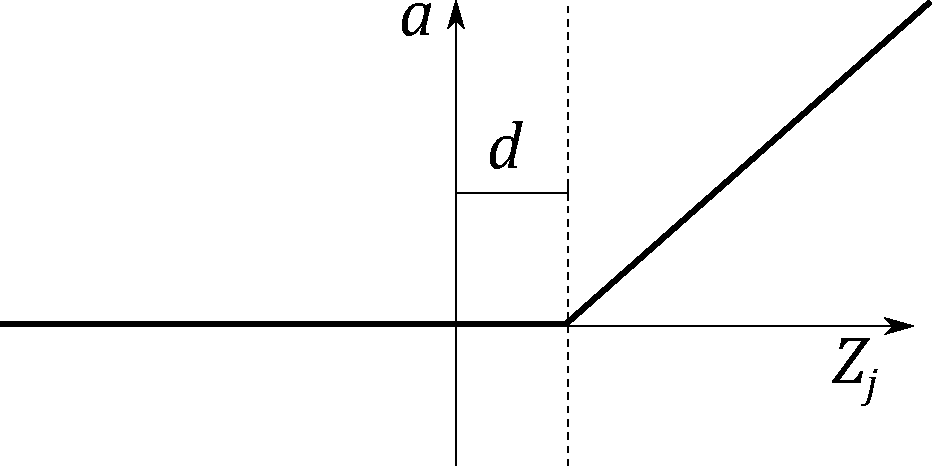
\includegraphics[width=0.5\linewidth]{images/relu.pdf}    

    \caption{In figure captions, explain what the reader is looking at: ``A schematic of the rectifying linear unit, where $a$ is the output amplitude,
    $d$ is a configurable dead-zone, and $Z_j$ is the input signal'', as well as why the reader is looking at this: 
    ``It is notable that there is no activation \emph{at all} below 0, which explains our initial results.'' 
    \textbf{Use vector image formats (.pdf) where possible}. Size figures appropriately, and do not make them over-large or too small to read.
    }

    % use the notation fig:name to cross reference a figure
    \label{fig:relu} 
\end{figure}


\begin{figure}
    \centering
    \begin{subfigure}[b]{0.45\textwidth}
        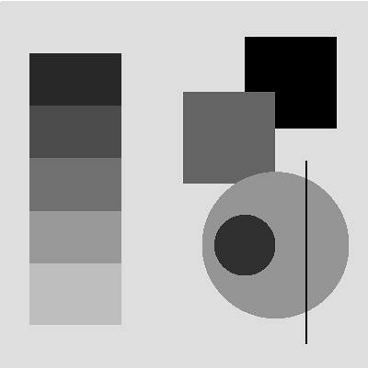
\includegraphics[width=\textwidth]{images/synthetic.png}
        \caption{Synthetic image, black on white.}
        \label{fig:syn1}
    \end{subfigure}
    ~ %add desired spacing between images, e. g. ~, \quad, \qquad, \hfill etc. 
      %(or a blank line to force the subfigure onto a new line)
    \begin{subfigure}[b]{0.45\textwidth}
        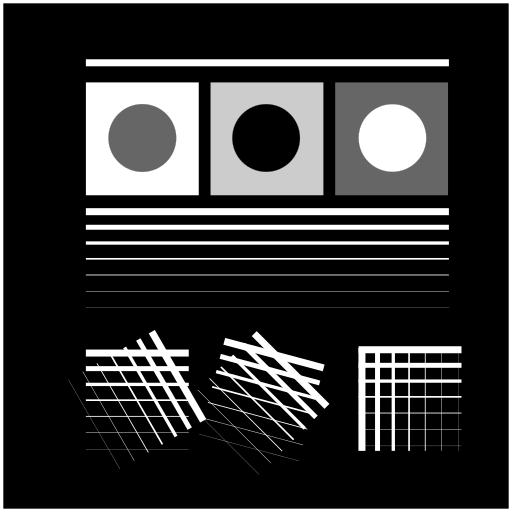
\includegraphics[width=\textwidth]{images/synthetic_2.png}
        \caption{Synthetic image, white on black.}
        \label{fig:syn2}
    \end{subfigure}
    ~ %add desired spacing between images, e. g. ~, \quad, \qquad, \hfill etc. 
    %(or a blank line to force the subfigure onto a new line)    
    \caption{Synthetic test images for edge detection algorithms. \subref{fig:syn1} shows various gray levels that require an adaptive algorithm. \subref{fig:syn2}
    shows more challenging edge detection tests that have crossing lines. Fusing these into full segments typically requires algorithms like the Hough transform.
    This is an example of using subfigures, with \texttt{subref}s in the caption.
    }\label{fig:synthetic}
\end{figure}

\clearpage

\subsection{Equations}

Equations should be typeset correctly and precisely. Make sure you get parenthesis sizing correct, and punctuate equations correctly 
(the comma is important and goes \textit{inside} the equation block). Explain any symbols used clearly if not defined earlier. 

For example, we might define:
\begin{equation}
    \hat{f}(\xi) = \frac{1}{2}\left[ \int_{-\infty}^{\infty} f(x) e^{2\pi i x \xi} \right],
\end{equation}    
where $\hat{f}(\xi)$ is the Fourier transform of the time domain signal $f(x)$.

\subsection{Algorithms}
Algorithms can be set using \texttt{algorithm2e}, as in Algorithm \ref{alg:metropolis}.

% NOTE: line ends are denoted by \; in algorithm2e
\begin{algorithm}
    \DontPrintSemicolon
    \KwData{$f_X(x)$, a probability density function returing the density at $x$.\; $\sigma$ a standard deviation specifying the spread of the proposal distribution.\;
    $x_0$, an initial starting condition.}
    \KwResult{$s=[x_1, x_2, \dots, x_n]$, $n$ samples approximately drawn from a distribution with PDF $f_X(x)$.}
    \Begin{
        $s \longleftarrow []$\;
        $p \longleftarrow f_X(x)$\;
        $i \longleftarrow 0$\;
        \While{$i < n$}
        {
            $x^\prime \longleftarrow \mathcal{N}(x, \sigma^2)$\;
            $p^\prime \longleftarrow f_X(x^\prime)$\;
            $a \longleftarrow \frac{p^\prime}{p}$\;
            $r \longleftarrow U(0,1)$\;
            \If{$r<a$}
            {
                $x \longleftarrow x^\prime$\;
                $p \longleftarrow f_X(x)$\;
                $i \longleftarrow i+1$\;
                append $x$ to $s$\;
            }
        }
    }
    
\caption{The Metropolis-Hastings MCMC algorithm for drawing samples from arbitrary probability distributions, 
specialised for normal proposal distributions $q(x^\prime|x) = \mathcal{N}(x, \sigma^2)$. The symmetry of the normal distribution means the acceptance rule takes the simplified form.}\label{alg:metropolis}
\end{algorithm}

\subsection{Tables}

If you need to include tables, like Table \ref{tab:operators}, use a tool like https://www.tablesgenerator.com/ to generate the table as it is
extremely tedious otherwise. 

\begin{table}[]
    \caption{The standard table of operators in Python, along with their functional equivalents from the \texttt{operator} package. Note that table
    captions go above the table, not below. Do not add additional rules/lines to tables. }\label{tab:operators}
    %\tt 
    \rowcolors{2}{}{gray!3}
    \begin{tabular}{@{}lll@{}}
    %\toprule
    \textbf{Operation}    & \textbf{Syntax}                & \textbf{Function}                            \\ %\midrule % optional rule for header
    Addition              & \texttt{a + b}                          & \texttt{add(a, b)}                                    \\
    Concatenation         & \texttt{seq1 + seq2}                    & \texttt{concat(seq1, seq2)}                           \\
    Containment Test      & \texttt{obj in seq}                     & \texttt{contains(seq, obj)}                           \\
    Division              & \texttt{a / b}                          & \texttt{div(a, b) }  \\
    Division              & \texttt{a / b}                          & \texttt{truediv(a, b) } \\
    Division              & \texttt{a // b}                         & \texttt{floordiv(a, b)}                               \\
    Bitwise And           & \texttt{a \& b}                         & \texttt{and\_(a, b)}                                  \\
    Bitwise Exclusive Or  & \texttt{a \textasciicircum b}           & \texttt{xor(a, b)}                                    \\
    Bitwise Inversion     & \texttt{$\sim$a}                        & \texttt{invert(a)}                                    \\
    Bitwise Or            & \texttt{a | b}                          & \texttt{or\_(a, b)}                                   \\
    Exponentiation        & \texttt{a ** b}                         & \texttt{pow(a, b)}                                    \\
    Identity              & \texttt{a is b}                         & \texttt{is\_(a, b)}                                   \\
    Identity              & \texttt{a is not b}                     & \texttt{is\_not(a, b)}                                \\
    Indexed Assignment    & \texttt{obj{[}k{]} = v}                 & \texttt{setitem(obj, k, v)}                           \\
    Indexed Deletion      & \texttt{del obj{[}k{]}}                 & \texttt{delitem(obj, k)}                              \\
    Indexing              & \texttt{obj{[}k{]}}                     & \texttt{getitem(obj, k)}                              \\
    Left Shift            & \texttt{a \textless{}\textless b}       & \texttt{lshift(a, b)}                                 \\
    Modulo                & \texttt{a \% b}                         & \texttt{mod(a, b)}                                    \\
    Multiplication        & \texttt{a * b}                          & \texttt{mul(a, b)}                                    \\
    Negation (Arithmetic) & \texttt{- a}                            & \texttt{neg(a)}                                       \\
    Negation (Logical)    & \texttt{not a}                          & \texttt{not\_(a)}                                     \\
    Positive              & \texttt{+ a}                            & \texttt{pos(a)}                                       \\
    Right Shift           & \texttt{a \textgreater{}\textgreater b} & \texttt{rshift(a, b)}                                 \\
    Sequence Repetition   & \texttt{seq * i}                        & \texttt{repeat(seq, i)}                               \\
    Slice Assignment      & \texttt{seq{[}i:j{]} = values}          & \texttt{setitem(seq, slice(i, j), values)}            \\
    Slice Deletion        & \texttt{del seq{[}i:j{]}}               & \texttt{delitem(seq, slice(i, j))}                    \\
    Slicing               & \texttt{seq{[}i:j{]}}                   & \texttt{getitem(seq, slice(i, j))}                    \\
    String Formatting     & \texttt{s \% obj}                       & \texttt{mod(s, obj)}                                  \\
    Subtraction           & \texttt{a - b}                          & \texttt{sub(a, b)}                                    \\
    Truth Test            & \texttt{obj}                            & \texttt{truth(obj)}                                   \\
    Ordering              & \texttt{a \textless b}                  & \texttt{lt(a, b)}                                     \\
    Ordering              & \texttt{a \textless{}= b}               & \texttt{le(a, b)}                                     \\
    % \bottomrule
    \end{tabular}
    \end{table}
\subsection{Code}

Avoid putting large blocks of code in the report (more than a page in one block, for example). Use syntax highlighting if possible, as in Listing \ref{lst:callahan}.

\begin{lstlisting}[language=python, float, caption={The algorithm for packing the $3\times 3$ outer-totalistic binary CA successor rule into a 
    $16\times 16\times 16\times 16$ 4 bit lookup table, running an equivalent, notionally 16-state $2\times 2$ CA.}, label=lst:callahan]
    def create_callahan_table(rule="b3s23"):
        """Generate the lookup table for the cells."""        
        s_table = np.zeros((16, 16, 16, 16), dtype=np.uint8)
        birth, survive = parse_rule(rule)

        # generate all 16 bit strings
        for iv in range(65536):
            bv = [(iv >> z) & 1 for z in range(16)]
            a, b, c, d, e, f, g, h, i, j, k, l, m, n, o, p = bv

            # compute next state of the inner 2x2
            nw = apply_rule(f, a, b, c, e, g, i, j, k)
            ne = apply_rule(g, b, c, d, f, h, j, k, l)
            sw = apply_rule(j, e, f, g, i, k, m, n, o)
            se = apply_rule(k, f, g, h, j, l, n, o, p)

            # compute the index of this 4x4
            nw_code = a | (b << 1) | (e << 2) | (f << 3)
            ne_code = c | (d << 1) | (g << 2) | (h << 3)
            sw_code = i | (j << 1) | (m << 2) | (n << 3)
            se_code = k | (l << 1) | (o << 2) | (p << 3)

            # compute the state for the 2x2
            next_code = nw | (ne << 1) | (sw << 2) | (se << 3)

            # get the 4x4 index, and write into the table
            s_table[nw_code, ne_code, sw_code, se_code] = next_code

        return s_table

\end{lstlisting}

%==================================================================================================================================
\chapter{Evaluation} 
How good is your solution? How well did you solve the general problem, and what evidence do you have to support that?

\section{Guidance}
\begin{itemize}
    \item
        Ask specific questions that address the general problem.
    \item
        Answer them with precise evidence (graphs, numbers, statistical
        analysis, qualitative analysis).
    \item
        Be fair and be scientific.
    \item
        The key thing is to show that you know how to evaluate your work, not
        that your work is the most amazing product ever.
\end{itemize}

\section{Evidence}
Make sure you present your evidence well. Use appropriate visualisations, 
reporting techniques and statistical analysis, as appropriate. The point is not
to dump all the data you have but to present an argument well supported by evidence gathered.

If you use numerical evidence, specify reasonable numbers of significant digits; don't state ``18.41141\% of users were successful'' if you only had 20 users. If you average \textit{anything}, present both a measure of central tendency (e.g. mean, median) \textit{and} a measure of spread (e.g. standard deviation, min/max, interquartile range).

You can use \texttt{siunitx} to define units, space numbers neatly, and set the precision for the whole LaTeX document. 

% setup siunitx to have two decimal places
\sisetup{
	round-mode = places,
	round-precision = 2
}

For example, these numbers will appear with two decimal places: \num{3.141592}, \num{2.71828}, and this one will appear with reasonable spacing \num{1000000}.



If you use statistical procedures, make sure you understand the process you are using,
and that you check the required assumptions hold in your case. 

If you visualise, follow the basic rules, as illustrated in Figure \ref{fig:boxplot}:
\begin{itemize}
\item Label everything correctly (axis, title, units).
\item Caption thoroughly.
\item Reference in text.
\item \textbf{Include appropriate display of uncertainty (e.g. error bars, Box plot)}
\item Minimize clutter.
\end{itemize}

See the file \texttt{guide\_to\_visualising.pdf} for further information and guidance.

\begin{figure}
    \centering
    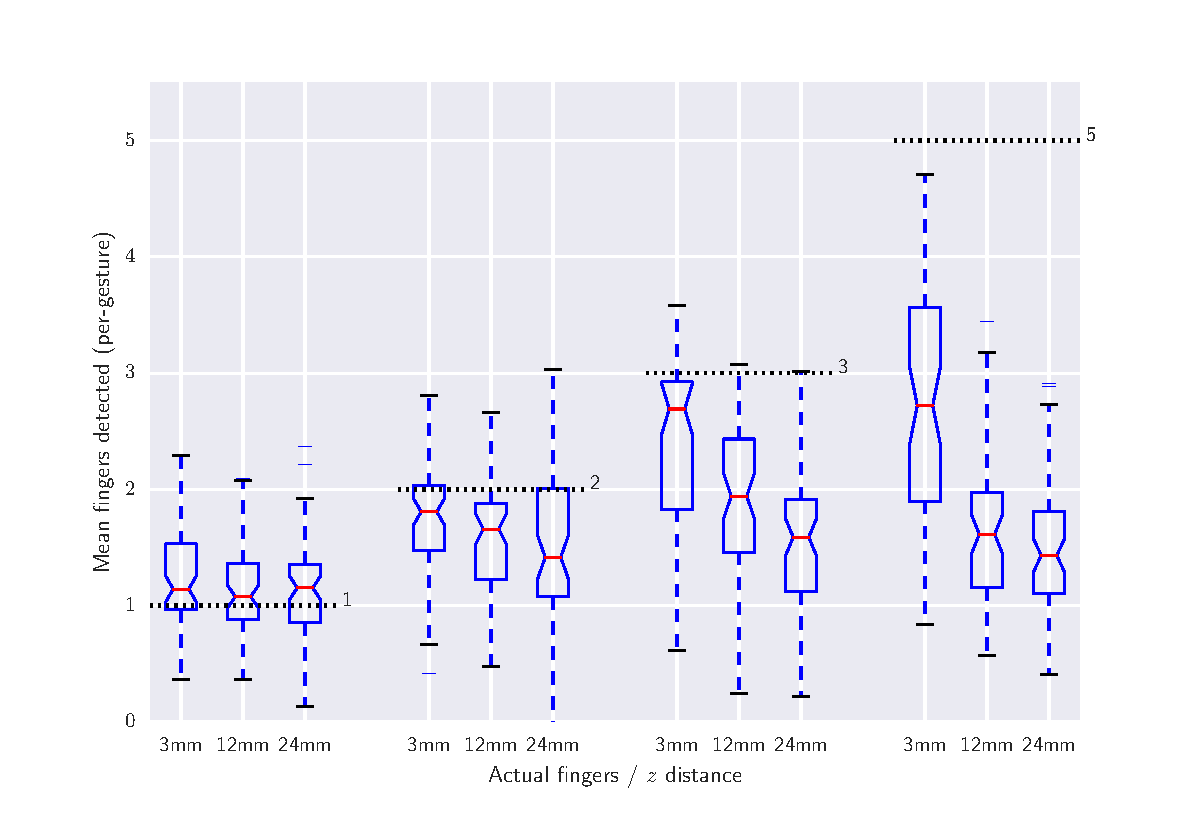
\includegraphics[width=1.0\linewidth]{images/boxplot_finger_distance.pdf}    

    \caption{Average number of fingers detected by the touch sensor at different heights above the surface, averaged over all gestures. Dashed lines indicate
    the true number of fingers present. The Box plots include bootstrapped uncertainty notches for the median. It is clear that the device is biased toward 
    undercounting fingers, particularly at higher $z$ distances.
    }

    % use the notation fig:name to cross reference a figure
    \label{fig:boxplot} 
\end{figure}


%==================================================================================================================================
\chapter{Conclusion}    
Summarise the whole project for a lazy reader who didn't read the rest (e.g. a prize-awarding committee). This chapter should be short in most dissertations; maybe one to three pages.
\section{Guidance}
\begin{itemize}
    \item
        Summarise briefly and fairly.
    \item
        You should be addressing the general problem you introduced in the
        Introduction.        
    \item
        Include summary of concrete results (``the new compiler ran 2x
        faster'')
    \item
        Indicate what future work could be done, but remember: \textbf{you
        won't get credit for things you haven't done}.
\end{itemize}

\section{Summary}
Summarise what you did; answer the general questions you asked in the introduction. What did you achieve? Briefly describe what was built and summarise the evaluation results.

\section{Reflection}
Discuss what went well and what didn't and how you would do things differently if you did this project again.

\section{Future work}
Discuss what you would do if you could take this further -- where would the interesting directions to go next be? (e.g. you got another year to work on it, or you started a company to work on this, or you pursued a PhD on this topic)

%==================================================================================================================================
%
% 
%==================================================================================================================================
%  APPENDICES  

\begin{appendices}

\chapter{Appendices}

Use separate appendix chapters for groups of ancillary material that support your dissertation. 
Typical inclusions in the appendices are:

\begin{itemize}
\item
  Copies of ethics approvals (you must include these if you needed to get them)
\item
  Copies of questionnaires etc. used to gather data from subjects. Don't include
  voluminous data logs; instead submit these electronically alongside your source code.
\item
  Extensive tables or figures that are too bulky to fit in the main body of
  the report, particularly ones that are repetitive and summarised in the body.
\item Outline of the source code (e.g. directory structure), 
    or other architecture documentation like class diagrams.
\item User manuals, and any guides to starting/running the software. 
Your equivalent of \texttt{readme.md} should be included.

\end{itemize}

\textbf{Don't include your source code in the appendices}. It will be
submitted separately.



\end{appendices}
%==================================================================================================================================
%   BIBLIOGRAPHY   

% The bibliography style is agsm (Harvard)
% The bibliography always appears last, after the appendices.

\bibliographystyle{agsm}

% Force the bibliography not to be numbered
\renewcommand{\thechapter}{0} 
\bibliography{l4proj}

\end{document}
